\chapter{\opal-env}

The \opalenv Envelope Tracker is an algorithm used to solve the envelope equations
of a beam propagating through external fields and under the influence of its
own space charge. The algorithm is based on the multi-slice analysis approach
used in the theory of emittance compensation \cite{bib:JBong}. The space charge
model used can be switched between an analytic model derived and used in HOMDYN
\cite{bib:HOMY} and a similar model developed at PSI called Beam Envelope Tracker
(BET).

\subsection{Envelope Equation without Dispersion For Long Beams}

The equation for the propagation of a general beam enveloped given here
follows the work of Sacherer \cite{Sach}. Using the variables $x$ and
$p_x$ as the phase space variables, the equation of motion for $\sigma_x =
\langle x^2\rangle^{1/2}$ is found by differentiating with respect to time:
%
\begin{eqnarray}
\dot\sigma_x = \frac{\langle x\dot x \rangle}{\sigma},\hspace{1cm}
\ddot\sigma_x = \frac{1}{\sigma_x^3}\left[\langle x^2\rangle \langle \dot x^2\rangle-\langle x\dot x\rangle^2\right]+\frac{\langle x\ddot x\rangle}{\sigma_x}
\end{eqnarray}
%
Noting that $\dot x = p_x/m\gamma$, the above equations become
%
\begin{eqnarray}
\ddot\sigma_x = \frac{1}{\sigma_x^3}\left(\frac{c\epsilon_n}{\gamma}\right)^2+\frac{\langle x\ddot x\rangle}{\sigma_x},
\end{eqnarray}
%
where the normalized emittance is defined as $\epsilon_{n,x} =
\frac{1}{mc}\sqrt{\langle x^2\rangle \langle p_x^2\rangle-\langle
xp_x\rangle^2}$. The last term in this equation is expanded using $\ddot x =
-\gamma^2\beta\dot\beta \dot x + F_x/m\gamma$:
%
\begin{eqnarray}
\ddot\sigma_x = \left[-\gamma^2\beta\dot\beta\right]\dot\sigma_x + \frac{\langle xF_x\rangle}{m\gamma\sigma_x}+\left(\frac{c\epsilon_n}{\gamma}\right)^2\frac{1}{\sigma_x^3},
\end{eqnarray}
%
The force is split into a (linear) external part and the self-fields: $F_x(t,x)
= -K_x(t)x + F_{x,s}$. Plugging this into the envelope equation gives
%
\begin{eqnarray}
\ddot\sigma_x + \left[\gamma^2\beta\dot\beta\right]\dot\sigma_x + \left[\frac{K}{m\gamma}\right]\sigma_x = \left[\frac{\langle xF_{x,s}\rangle}{m\gamma}\right]\frac{1}{\sigma_x}+\left(\frac{c\epsilon_n}{\gamma}\right)^2\frac{1}{\sigma_x^3}.
\end{eqnarray}
%
Following Sacherer \cite{Sach}, the term $\langle xF_{x,s}\rangle$ can be
interpreted as the linear part of the space charge field (in a least squares
sense). The linear part of the field is defined by $F_{x,s}^{(1)}$, such that
the quantity
%
\begin{eqnarray}
D = \langle (F_{x,s}^{(1)}x-F_{x,s})^2\rangle = \int (F_{x,s}^{(1)}x-F_{x,s})^2\rho_x\;\differential{}x,
\end{eqnarray}
%
is minimized in a least squares sense. This is accomplished by setting $\pdifferential{}D / \pdifferential{} F_{x,s}^{(1)} = 0$, which implies \cite{Sach}:
%
\begin{eqnarray}
F_{x,s}^{(1)}x = \frac{\langle xF_{x,s}\rangle}{\sigma_x^2}x.
\end{eqnarray}
%
This gives the general form of the envelope equation
%
\begin{eqnarray}
\ddot\sigma_x + \left[\gamma^2\beta\dot\beta\right]\dot\sigma_x
+ \left[\frac{K}{m\gamma}\right]\sigma_x &=& \left[\frac{F_{x,s}^{(1)}}{m\gamma}\right]\sigma_x+\left(\frac{c\epsilon_n}{\gamma}\right)^2\frac{1}{\sigma_x^3},
\nonumber
\\
\sigma_x\nprimed{2} + \left[\frac{\gamma\primed}{\beta^2\gamma}\right]\sigma_x\primed + \left[\frac{K}{mc^2\beta p_n}\right]\sigma_x &=& \left[\frac{F_{x,s}^{(1)}}{mc^2\beta p_n}\right]\sigma_x+\left(\frac{\epsilon_n}{p_n}\right)^2\frac{1}{\sigma_x^3}.
\end{eqnarray}
%
In this equation $p_n = \beta\gamma$ is the normalized momentum.

A general form for the fields can be now introduced. For a long beam, the linear
part of the fields (in the beam rest frame) are given by
%
\begin{eqnarray}
E_x=\left( \left.\diffp{E_x}{x}\right|_{0}\right)x,\hspace{1cm}E_y= \left(\left.\diffp{E_y}{y}\right|_{0}\right)y.
\end{eqnarray}
%
These fields must then be boosted back to the laboratory frame according to
%
\begin{eqnarray}
\textbf{E}&=&\gamma(\textbf{E}\primed-\vec{\mathbf{\beta}}\times
c\textbf{B}\primed)-\frac{\gamma^2}{1+\gamma}\vec{\beta}(\vec{\beta}\cdot
\textbf{E}\primed),\nonumber
\\
\textbf{B}&=&\gamma(\textbf{B}\primed+\vec{\mathbf{\beta}}\times
\textbf{E}\primed/c)-\frac{\gamma^2}{1+\gamma}\vec{\beta}(\vec{\beta}\cdot
\textbf{B}\primed),\label{eq:FieldTrans}
\end{eqnarray}
%
For a beam moving along the $z$-axis with speed $c\beta$, the fields are given by
%
\begin{eqnarray}
\mathbf{E} = \gamma E_x\primed\hat{\mathbf{x}} + \gamma E_y\primed\hat{\mathbf{y}}, \hspace{2cm}
\mathbf{B} = \frac{\gamma\beta}{c}(-E_y\primed\hat{\mathbf{x}} + E_x\primed\hat{\mathbf{y}}).
\end{eqnarray}
%
Here the primes label the field components in the lab frame. Assuming these
components are proportional to the line charge density $\lambda\primed$ the
fields can be written in a form that takes into account the Lorentz contraction
of the current density:
%
\begin{eqnarray}
E_x = \gamma E_x\primed = \gamma\lambda\primed\diffp{E_x\primed}{\lambda\primed}=\lambda\diffp{E_x\primed}{\lambda\primed}.
\end{eqnarray}
%
The linearized force equation then takes the form
%\begin{eqnarray}
%\mathbf{F} = e(E_r-\beta c B_{\theta})\hat{\mathbf{r}} = \frac{e\lambda}{\gamma^2}\left(\diffp{E_r\primed}{{r}{\lambda\primed}}\right) r\hat{\mathbf{r}}
%\end{eqnarray}
%
\begin{eqnarray}
\mathbf{F} &=& e(E_x-\beta c B_{y})\hat{\mathbf{x}} + e(E_y + \beta c B_{x})\hat{\mathbf{y}}
\nonumber
%\\
 %&=&
  = \frac{e\lambda}{\gamma^2}
 \left[
 \left(\diffp{E_x\primed}{{x}{\lambda\primed}}\right) x \hat{\mathbf{x}}+
 \left(\diffp{E_y\primed}{{y}{\lambda\primed}}\right) y \hat{\mathbf{y}}
\right].
\end{eqnarray}
%
With this, the envelope equations become
%
\begin{eqnarray}
\ddot\sigma_i + \left[\gamma^2\beta\dot\beta\right]\dot\sigma_i
+ \left[\frac{K_i}{m\gamma}\right]\sigma_i &=& \left[\frac{e\lambda}{m\gamma^3}\left(\diffp{E_i\primed}{{x_i}{\lambda\primed}}\right)\right]\sigma_i+\left(\frac{c\epsilon_{n,i}}{\gamma}\right)^2\frac{1}{\sigma_i^3}.
%\nonumber
%\\
%\sigma_i\nprimed{2} + \left[\frac{\gamma\primed}{\beta^2\gamma}\right]\sigma_i\primed + \left[\frac{K_i}{mc^2\beta p_n}\right]\sigma_i &=& \left[\frac{e\lambda}{mc^2\beta^2  \gamma^3}\left(\diffp{E_i\primed}{{x_i}{\lambda\primed}}\right)\right]\sigma_i+\left(\frac{\epsilon_{n,i}}{p_n}\right)^2\frac{1}{\sigma_i^3}.
\label{eq:GenEnv}
\end{eqnarray}


So far this derivation has assumed that there is no coupling between $x$ and
$y$ in both the external and self forces. In the presence of solenoids this is
no longer the case for the external fields. If the beam and external fields
are cylindrical symmetric then the previous analysis can be performed in the
Larmor frame. Working in the Larmor frame, the equations of motion for $\sigma_x
=\sigma_y =\sigma_L$ decouple and the envelope equation is given by
%
\begin{eqnarray}
\ddot\sigma_L + \left[\gamma^2\beta\dot\beta\right]\dot\sigma_L + \left[\frac{K}{m\gamma}+(\dot\theta_r)^2\right]\sigma_L &=& \left[\frac{e\lambda}{m \gamma^3}\left(\diffp{E_r\primed}{{r}{\lambda\primed}}\right)\right]\sigma_L+\left(\frac{c\epsilon_n}{\gamma}\right)^2\frac{1}{\sigma_L^3}.
\nonumber
%\\
%\sigma\nprimed{2} + \left[\frac{\gamma\primed}{\beta^2\gamma}\right]\sigma\primed
%+ \left[\frac{K}{mc^2\beta p_n} + (\theta_r\primed)^2\right]\sigma &=&
%\left[\frac{e\lambda}{mc^2\beta^2 \gamma^3}\left(\diffp{E_r\primed}{{r}{\lambda\primed}}\right)\right]\sigma+\left(\frac{\epsilon_n}{p_n}\right)^2\frac{1}{\sigma^3}.
\end{eqnarray}
%
In this expression, $\theta_r$ is the Larmor angle, and is given by
%
\begin{eqnarray}
\theta_r  = -\int\left(\frac{eB_z}{2m\gamma }\right)\;\differential{}t = -\int\left(\frac{eB_z}{2m\gamma \beta c}\right)\;\differential{}z.
\end{eqnarray}

\subsubsection{Long Uniform Cylindrical Beam}

The envelope equation for a cylindrical beam is now explicitly derived. Assuming
cylindrical symmetric fields and working in the Larmor frame then $\sigma_x
= \sigma_y = \sigma_L$. It is important to distinguish this parameter from $
\sigma_r = R/\sqrt{2}$. In fact, $\sigma_L = R/2$ for a circular beam. The
electric in the lab frame can be easily computed from Gauss's law:
%
\begin{eqnarray}
E_r\primed = \frac{1}{8\pi\epsilon_0}\frac{\lambda\primed}{\sigma^2}r  \hspace{1cm} (r<R).
\end{eqnarray}
%
This is the only portion of the field needed since the charge is zero outside of
the cylinder radius, and the average $\langle xF_x\rangle$ is zero there. The
space charge term is then given by
%
\begin{eqnarray}
\frac{e\lambda}{m\gamma^3}\left(\diffp{E_r\primed}{{r}{\lambda\primed}}\right)
=\frac{c^2}{2\beta\sigma^2}\left(\frac{e}{4\pi\epsilon_0mc^3}\right)\lambda\beta c = \frac{c^2}{\beta\sigma^2}\frac{I}{2I_0},
\end{eqnarray}
%
where the Alfven current is identified as the factors in parenthesis. With this
the envelope equation is written in its `standard' form \cite{bib:JBong}
%
\begin{eqnarray}
\ddot\sigma_L + \left[\gamma^2\beta\dot\beta\right]\dot\sigma_L + \left[\frac{K}{m\gamma}+(\dot\theta_r)^2\right]\sigma_L &=&
\left[\frac{c^2k_p}{\beta \gamma^3}\right]\frac{1}{\sigma_L}+\left(\frac{c\epsilon_n}{\gamma}\right)^2\frac{1}{\sigma_L^3},
\nonumber
%\\
%\sigma\nprimed{2} + \left[\frac{\gamma\primed}{\beta^2\gamma}\right]\sigma\primed
%+ \left[\frac{K}{mc^2\beta p_n} + (\theta_r\primed)^2\right]\sigma &=&
%\left[\frac{k_p}{p_n^3}\right]\frac{1}{\sigma}+\left(\frac{\epsilon_n}{p_n}\right)^2\frac{1}{\sigma^3},
\end{eqnarray}
%
where the term $k_p = I/2I_0$ is the beam perveance. Equivalently, these
equations can be written in terms of the beam radius $R$:
%
\begin{eqnarray}
\ddot R + \left[\gamma^2\beta\dot\beta\right]\dot R + \left[\frac{K}{m\gamma}+(\dot\theta_r)^2\right]R&=&
\left[\frac{4c^2k_p}{\beta \gamma^3}\right]\frac{1}{R}+\left(\frac{4c\epsilon_n}{\gamma}\right)^2\frac{1}{R^3}.
%\nonumber
%\\
%R\nprimed{2} + \left[\frac{\gamma\primed}{\beta^2\gamma}\right]R\primed
%+ \left[\frac{K}{mc^2\beta p_n} + (\theta_r\primed)^2\right]R &=&
%\left[\frac{4k_p}{p_n^3}\right]\frac{1}{R}+\left(\frac{4\epsilon_n}{p_n}\right)^2\frac{1}{R^3}.
\end{eqnarray}

\subsubsection{Long Uniform Elliptical Beam}

Here an intuitive argument is used to find the linear portions of the fields
from a uniform elliptical beam. The beam's cross-section is defined so that the
ellipse axes line up with the $x$ and $y$ Cartesian coordinates and are given by
$X$ and $Y$ respectively. The symmetry of the problem in Cartesian coordinates
implies the following constraints on the transverse electric field components in
the beam rest frame:
%
\begin{eqnarray}
\left\{
\begin{array}{c}
E_x(-x,y,z) = -E_x(x,y,z) \\
E_x(x,-y,z) = \hspace{0.3cm}E_x(x,y,z)
\end{array}
\right. ,
\hspace{1cm}
\left\{
\begin{array}{c}
E_y(-x,y,z) = \hspace{0.3cm}E_y(x,y,z) \\
E_y(x,-y,z) = -E_y(x,y,z)\end{array}
\right. ,
\end{eqnarray}
%
These conditions imply that field components can be expanded as
%
\begin{eqnarray}
E_x = \sum_{n,m=0}^{\infty}E_x^{(2n+1,2m)}x^{2n+1}y^{2m},\hspace{1cm}E_y = \sum_{n,m=0}^{\infty}E_y^{(2n,2m+1)}x^{2n}y^{2m+1}.
\end{eqnarray}
%
Similarly the charge density must satisfy $\rho(-x,-y) = \rho(x,y)$, implying:
%
\begin{eqnarray}
\rho(x,y) = \sum_{n,m=0}^{\infty}\rho^{(2n,2m)}x^{2n}y^{2m}.
\end{eqnarray}
%
Gauss's law can then be use to relate the expansion coefficients:
%
\begin{eqnarray}
(2n+1)E_x^{(2n+1,2m)} + (2m+1)E_y^{(2n, 2m+1)} = \frac{1}{\epsilon_0}\rho^{(2n,2m)}
\end{eqnarray}
%
The linear components of the field (inside the beam) are given by taking
$n=m=0$. This implies that
%
\begin{eqnarray}
\left.\diffp{E_x}{x}\right|_{r=0} + \left.\diffp{E_y}{y}\right|_{r=0} = \frac{\lambda}{\pi\epsilon_0XY}.
\end{eqnarray}
%
It is now assumed that for the linear portion of the fields, the above
derivatives have a similar form. The assumed form is
%
\begin{eqnarray}
\left.\diffp{E_x}{x}\right|_{r=0} = \frac{f}{X},\hspace{1cm} \left.\diffp{E_y}{y}\right|_{r=0}=\frac{f}{Y}.
\end{eqnarray}
%
The form here is chosen so that the field components have the right behavior in
the limit that $X$ or $Y$ goes to zero, as well as the limit $X=Y=R$. With this
assumption, the linear field components can be solved for:
%
\begin{eqnarray}
E_x = \frac{\lambda x}{\pi\epsilon_0X(X+Y)},\hspace{1cm} E_y = \frac{\lambda y}{\pi\epsilon_0Y(X+Y)}.
\end{eqnarray}
%
For a more rigorous derivation of this result, please see \cite{Sach}.
From these expressions the envelope equations can be derived using \eqnref{GenEnv}:
%
\begin{eqnarray}
\ddot\sigma_i + \left[\gamma^2\beta\dot\beta\right]\dot\sigma_i
+ \left[\frac{K_i}{m\gamma}\right]\sigma_i &=& \left[\frac{2c^2}{\beta\gamma^3}\right]\frac{k_p}{\sigma_x+\sigma_y}+\left(\frac{c\epsilon_{n,i}}{\gamma}\right)^2\frac{1}{\sigma_i^3}.
%\nonumber
%,\\
%\sigma_i\nprimed{2} + \left[\frac{\gamma\primed}{\beta^2\gamma}\right]\sigma_i\primed + \left[\frac{K_i}{mc^2\beta p_n}\right]\sigma_i &=& \left[\frac{2}{p_n^3}\right]\frac{k_p}{\sigma_x+\sigma_y}+\left(\frac{\epsilon_{n,i}}{p_n}\right)^2\frac{1}{\sigma_i^3}.
\end{eqnarray}
%
The equivalent equations for the ellipse axes are the given by
%
\begin{eqnarray}
\ddot X_i + \left[\gamma^2\beta\dot\beta\right]\dot X_i
+ \left[\frac{K_i}{m\gamma}\right]X_i &=& \left[\frac{8c^2}{\beta\gamma^3}\right]\frac{k_p}{X+Y}+\left(\frac{4c\epsilon_{n,i}}{\gamma}\right)^2\frac{1}{X_i^3}.
%\nonumber
%\\
%X_i\nprimed{2} + \left[\frac{\gamma\primed}{\beta^2\gamma}\right]X_i\primed + \left[\frac{K_i}{mc^2\beta p_n}\right]X_i &=& \left[\frac{8}{p_n^3}\right]\frac{k_p}{X+Y}+\left(\frac{4\epsilon_{n,i}}{p_n}\right)^2\frac{1}{X_i^3}.
\end{eqnarray}

\subsection{Slice Model}

The slice model deployed in \opalenv is based on the slice analysis of the
envelope equation developed in emittance compensation theory \cite{bib:JBong}.
In this analysis the beam is taken to be laminar in both the transverse and
longitudinal directions. The beam is then cut into slices along the length of
the bunch. The slices are taken to be independent, and the transverse envelope
equation applied to each.
%
\begin{figure}[h]
  \begin{center}
        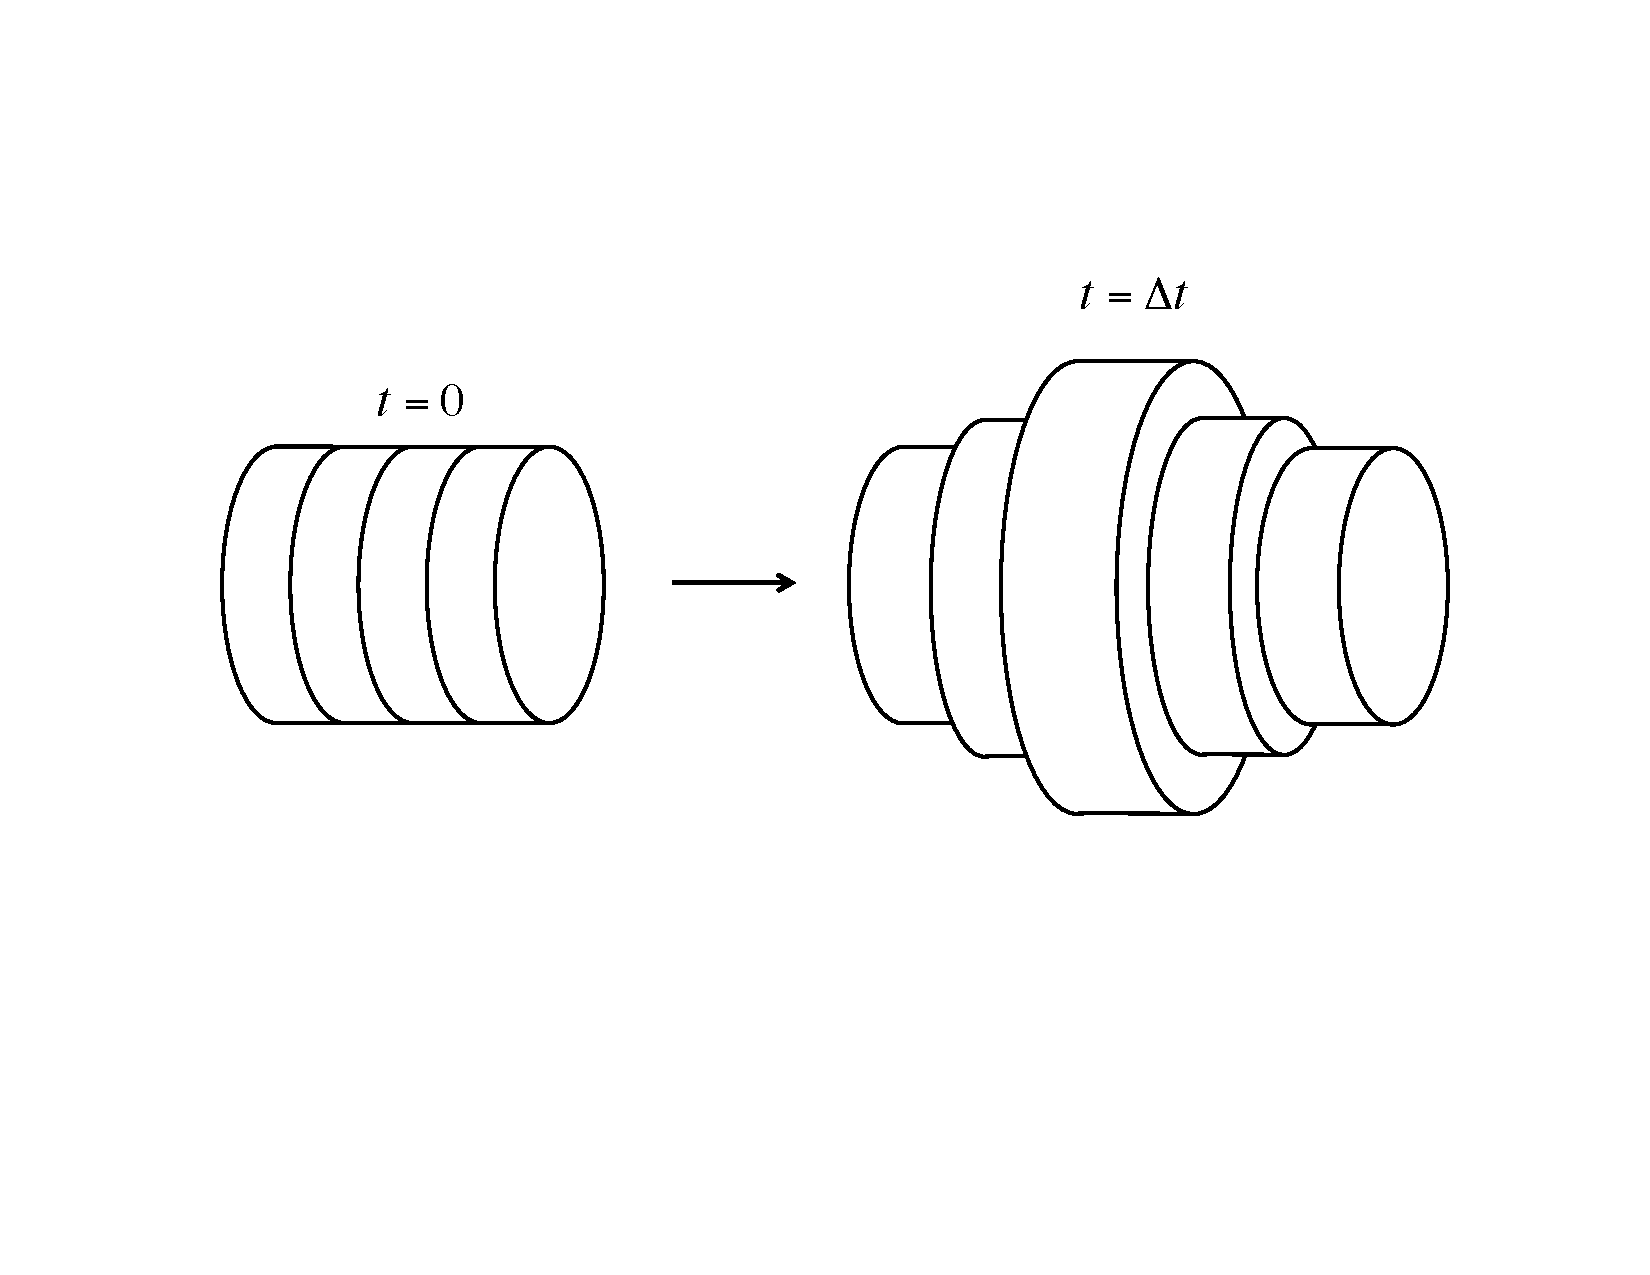
\includegraphics[width=120mm]{figures/HomdynPlots1}
        \caption{Evolution of the particle beam in the multi-slice approximation.}
    \label{fig:sliceModel}
  \end{center}
\end{figure}
%
As a result, each slice changes both in length and radius as the beam
propagates through the accelerator. This is shown schematically in
\figref{sliceModel}. The position of each slice is labeled by the
coordinate $\zeta$. The beam envelope of each slice is then written as
$\sigma = \sigma(t,z,\zeta)$.
Additionally, for very long beams, the current is given by
%
\begin{eqnarray}
I = I(t,z,\zeta) = c\beta(\zeta)\lambda(\zeta).
\end{eqnarray}
%
In the case of bunched beams, the current picks up an extra factor:
%
\begin{eqnarray}
I\rightarrow I(\zeta)g(\zeta).  \label{eq:FormFact}
\end{eqnarray}
%
The term $g(\zeta)$ is determined by the bunch distribution, and is less than or
equal to unity. It is noted that in this model the slices are assumed to have
some infinitesimal width $\delta\zeta = \delta\zeta(t,z)$ which is the same
for all slices. For a bunched beam with length L this is given by $\delta\zeta
= L/N$, where $N$ is the number of slices. The position of each slice evolves
according
%
\begin{eqnarray}
\dot\beta(t,\zeta) = \frac{eE_z}{mc\gamma^3(\zeta)}.
\end{eqnarray}
%
The longitudinal field here includes both the external and self-fields (for
bunched beams) at the slice position.
%The space charge force of each slice is approximated by assuming that each slice
%is a uniformly filled cylinder of charge. An approximate form for the fields can
%then be found.

\subsubsection{The HOMDYN Model: Analytic Space Charge Fields for Bunched Beams}

In this section the analytic formula for the linear Electric fields fields
from a uniformly charged cylinder are derived. This done in two steps. First
the on-axis field from a uniformly charged circular disk is calculated. The
infinitesimal field contribution in this case is
%
\begin{eqnarray}
d\mathbf{E} =
\frac{1}{4\pi\epsilon_0}\frac{(\mathbf{x}-\mathbf{x}\primed)}
{|\mathbf{x}-\mathbf{x}\primed|^3}\sigma dA\primed,\nonumber
\end{eqnarray}
%
with $\mathbf{x}-\mathbf{x}\primed=
(z-z\primed)\hat{\mathbf{z}}-r\primed\hat{\mathbf{r}}\primed$ on-axis.
Noting that the integration over the radial component vanishes on-axis, the
field from the disk can be readily integrated, yielding:
%
\begin{eqnarray}
\mathbf{E}_{z}^{\textmd{disk}}(r=0) &=&
\frac{\sigma}{2\epsilon_0}
\left(\frac{(z-z\primed)}{|z-z\primed|}-\frac{(z-z\primed)}{\sqrt{(z-z\primed)^2+R^2}}\right)\hat{\mathbf{z}}.
\end{eqnarray}
%
From this, the on-axis field for the cylinder can be found by letting $\sigma
= \rho_0dz\primed$ and integrating up the contribution from infinitesimal
charged disks from $0\leq z\primed\leq L$:
%
%\begin{equation}
%\mathbf{E}_z(r=0)=\frac{Q}{2\pi\epsilon_0R^2}
%\left(\sqrt{(1-z/L)^2+(R/L)^2}-\sqrt{z^2+R^2}-|L-z|+|z|\right)\hat{\mathbf{z}}.
%\nonumber
%\end{equation}
%
%This can be written more compactly as
%
\begin{eqnarray}
{E}_z(=0)&=&\frac{Q}{2\pi\epsilon_0R^2}H(z,A),
\end{eqnarray}
%
where the function $H(z,A)$ is given by
%
\begin{eqnarray}
H(z,A) = \sqrt{\left(1-\frac{z}{L} \right)^2+A^2}-\sqrt{\left(\frac{z}{L}\right)^2 +A^2}
-\left|1-\frac{z}{L}\right| +\left|\frac{z}{L}\right|,\hspace{0.5cm}A = R/L.
\end{eqnarray}

Using Maxwell's equations allows one to find $E_{r}$. For cylindrical symmetry,
Gauss's law takes the form
%
\begin{eqnarray}
\diffp{}{r}(r E_{r}) =
r\left(\frac{\rho_0}{\epsilon_0}-\diffp{E_z}{z}\right),\label{eq:FindErho}
%\cong
r\left(\frac{\rho(r,z)}{\epsilon_0}-\diff{}{z}E_z(0,z)\right),
\nonumber
\end{eqnarray}
%
where the charge density $\rho = \rho_0[\theta_H(r)-\theta_H(r-R)]\cdot
[\theta_H(z)-\theta_H(z-L)]$. Approximating Gauss's law to first order in $r$
gives
%
\begin{eqnarray}
\diffp{}{r}(r E_{r}) =
r\left(\frac{\rho_0}{\epsilon_0}[\theta_H(z)-\theta_H(z-L)]-\frac{d E_z} {dz}(r=0)\right).
\end{eqnarray}
%
The derivative $dE_z/dz$ is given by
%
\begin{eqnarray}
\frac{d}{dz}E_z(0,z) = \frac{\rho_0}{2\epsilon_0}
\left(\frac{z-L}{\sqrt{(z-L)^2+R^2}}
-\frac{z}{\sqrt{z^2+R^2}} + 2\left[\theta_H(z)-\theta_H(z-L)\right]
\right).
\end{eqnarray}
%
Plugging this expression into Gauss's law then yields
%
\begin{eqnarray}
\diffp{}{r}(r E_{r})\cong r \frac{\rho_0}{2\epsilon_0}
\left(\frac{L-z}{\sqrt{(L-z)^2+R^2}}+\frac{z}{\sqrt{z^2+R^2}}\right).
\end{eqnarray}
%
Thus the radial component is given to first order in $r$ as
%
\begin{eqnarray}
E_{r}=r\frac{\rho_0}{4\epsilon_0}
\left(\frac{L-z}{\sqrt{(L-z)^2+R^2}}+\frac{z}{\sqrt{z^2+R^2}}\right)r.\nonumber
\end{eqnarray}
%
This can be written as
%
\begin{eqnarray}
E_{r}=\frac{Qr}{4\pi\epsilon_0R^2L}
\left(\frac{1-z/L}{\sqrt{(1-z/L)^2+(R/L)^2}}+\frac{z/L}{\sqrt{(z/L)^2+(R/L)^2}}\right)
\end{eqnarray}
%
This is written more compactly as
%
\begin{eqnarray}
E_{r}=\frac{Qr}{4\pi\epsilon_0R^2L}G(z,A).
\end{eqnarray}
%
where $G(z,A)$ is the term in parenthesis and $A=R/L$ is the aspect ratio of the
cylinder. For a moving cylinder of charge, these fields must be boosted back
to the lab frame. This is accomplished using \eqnref{FieldTrans}. If the
cylinder is moving down the $z$-axis with a velocity given by $\dot z=c\beta$,
the transformation is the same as before, except now there is a $z$ component to
the electric field $E_z = E_z\primed$. Remembering to include the contraction
effect on the length of the cylinder ($z\rightarrow \gamma z$ and $L\rightarrow
\gamma L $), the fields can be written as
%
\begin{eqnarray}
E_z = \frac{Q}{2\pi\epsilon_0R^2} H(\zeta, A), \hspace{0.5cm} E_r \frac{Qr}{4\pi\epsilon_0R^2L} G(\zeta, A), \hspace{0.5cm}
B_{\theta} = \frac{\beta}{c}E_r,
\end{eqnarray}
%
where the tail of the cylinder is $z_t$ and $\zeta = z - z_{t}$. The functions
$H$ and $G$ have been previously defined. In this expression $A = R/\gamma L$.

The envelope equation can be written down for the propagation for each slice
by assuming the space charge force from the bunch is approximately the same as
the space charge force from a uniform cylinder with charge and length given by
the full bunch charge and length, but with a radius given by the slice radius.
Identifying the $\lambda = Q/L\primed$ in the beam rest frame, the first order
component of the transverse fields can be written as
%
\begin{eqnarray}
E_r^{\prime(1)}= \frac{\lambda\primed}{8\pi\epsilon_0\sigma^2}\left[\frac{G(\zeta\primed,A\primed)}{2}\right].
\end{eqnarray}
%
Following the previous analysis, the envelope equation then becomes
%
\begin{eqnarray}
\ddot\sigma + \left[\gamma^2\beta\dot\beta\right]\dot\sigma + \left[\frac{K}{m\gamma}+(\dot\theta_r)^2\right]\sigma &=&
\left[\frac{c^2k_p}{\beta \gamma^3}\left(\frac{G(\zeta,A)}{2}\right)\right]\frac{1}{\sigma}+\left(\frac{c\epsilon_n}{\gamma}\right)^2\frac{1}{\sigma^3},
\nonumber
%\\
%\sigma\nprimed{2} + \left[\frac{\gamma\primed}{\beta^2\gamma}\right]\sigma\primed
%+ \left[\frac{K}{mc^2\beta p_n} + (\theta_r\primed)^2\right]\sigma &=&
%\left[\frac{k_p}{p_n^3}\left(\frac{G(\zeta,A)}{2}\right)\right]\frac{1}{\sigma}+\left(\frac{\epsilon_n}{p_n}\right)^2\frac{1}{\sigma^3}.
\end{eqnarray}
%
Explicitly, the perveance term is written out as
%
\begin{eqnarray}
K = \frac{I}{2I_0}\cdot \frac{G}{2} = c\beta(\zeta)\left(\frac{Q}{L}\right)\left(\frac{G(\zeta,A)}{2}\right).
\end{eqnarray}
%
This is exactly the form for the current described in the previous section.
The function $G(\zeta,A)/2$ is identified as the form factor term $g(\zeta)$
in \eqnref{FormFact}. \figref{gmoney} shows the the function
$G(\zeta,A)/2$ for various values of the aspect ratio $A = R/L/\gamma$.
%
\begin{figure}[h]
  \begin{center}
        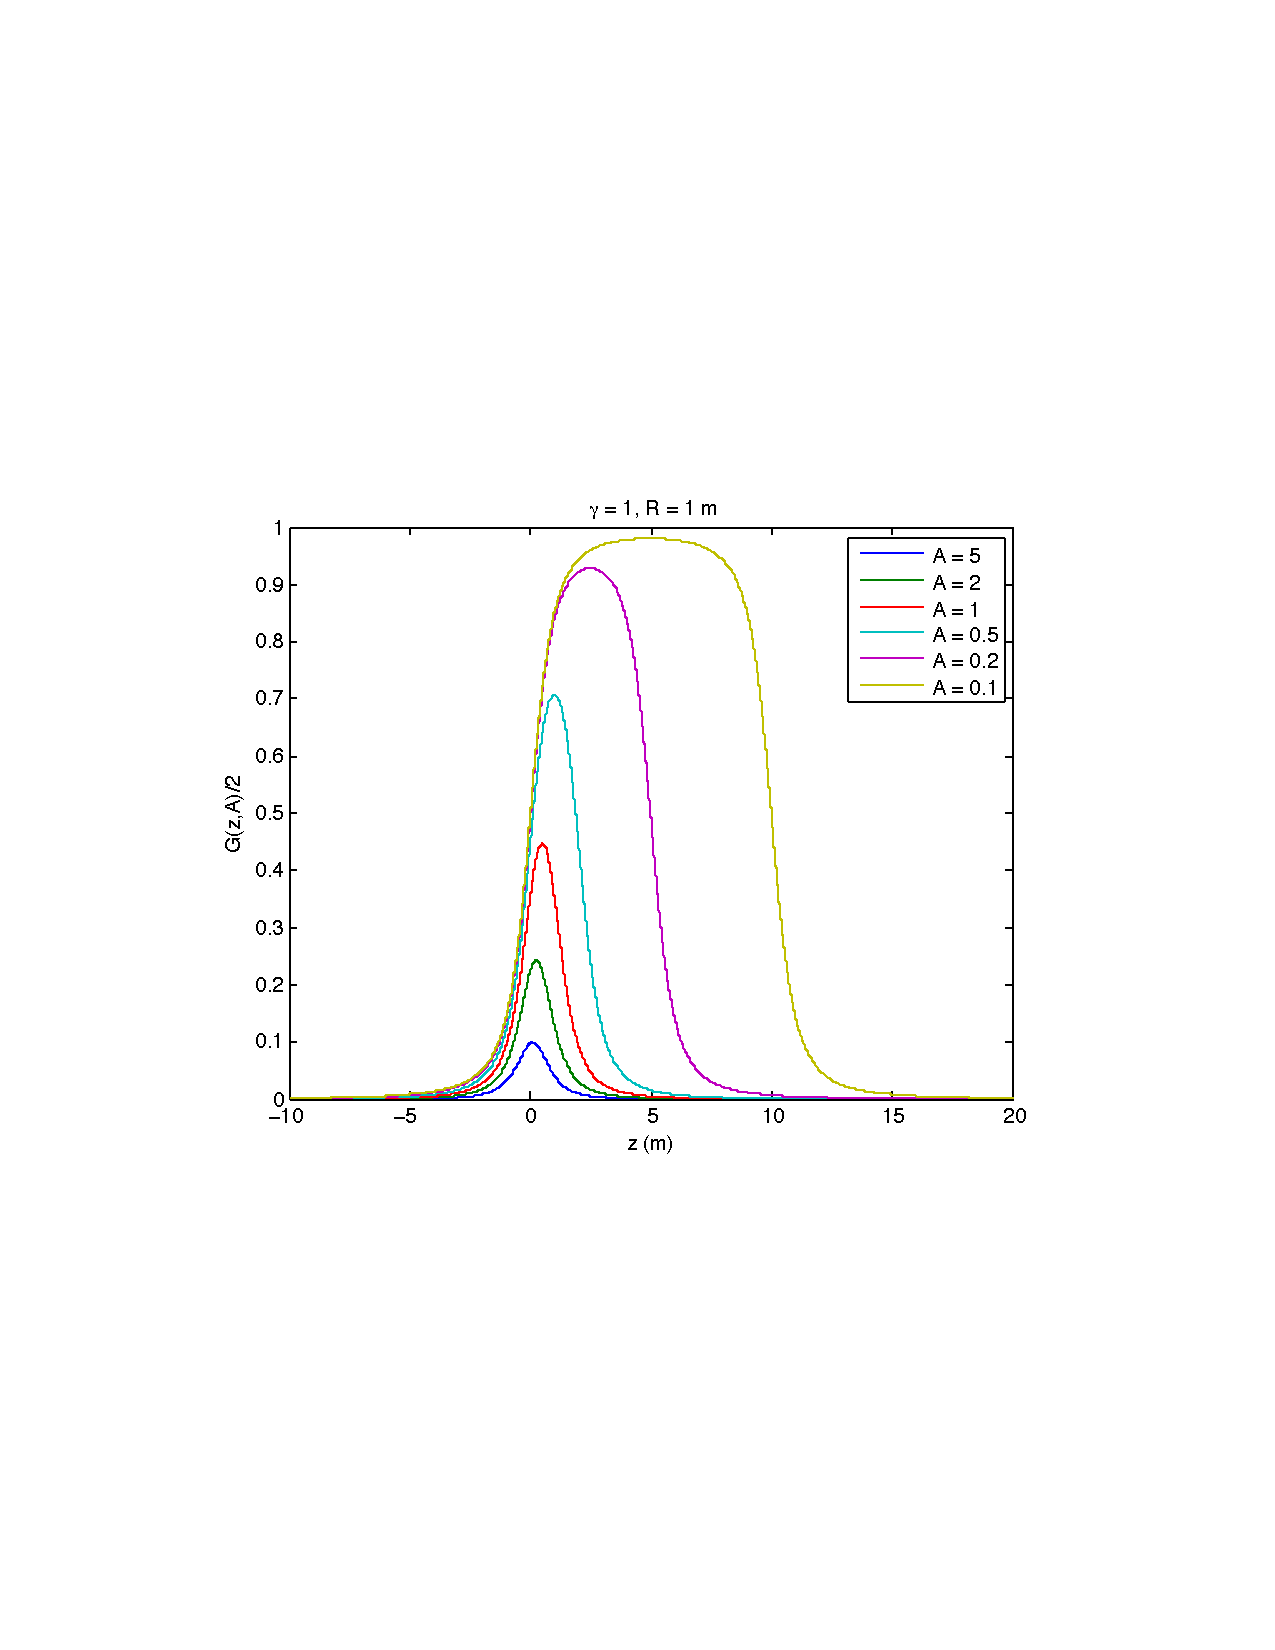
\includegraphics[width=120mm]{figures/Gfact}
        \caption{The bunch form factor $g(\zeta) = G(\zeta,A)/2$.}
    \label{fig:gmoney}
  \end{center}
\end{figure}
%
As the figure shows the form factor is less than or equal to unity.

It turns out that this form factor can also be used to describe elliptical beams
as well. For long beams, the space charge fields on envelope from an elliptical
beam are equivalent to those of a circular beam with a effective radius $R^{*} =
(X+Y)/2$. This equivalence gives a good approximation for bunched beams as well
\cite{HOMY2}. For writing down the final envelope equations, the effect of image
charges (for emission from a cathode) are included. This is done by letting
%
\begin{eqnarray}
\frac{I(\zeta)g(\zeta)}{\gamma^2}\rightarrow I(\zeta)[(1-\beta^2)g(\zeta) - (1+\beta^2)g(\xi) ],\nonumber
\end{eqnarray}
%
where $\xi = z_s + z_h$. Effectively, this just includes a mirror bunch behind
the cathode. With this, the final equations of motion for the HOMDYN algorithm
are written collected together. For the case of a cylindrical system, the
equations are given in the Larmor frame as:
%
\begin{eqnarray}
\lefteqn{\ddot\sigma_L + \left[\gamma^2\beta\dot\beta\right]\dot\sigma_L + \left[\frac{K}{m\gamma}+(\dot\theta_r)^2\right]\sigma_L=} & &
\nonumber
\\
& & \hspace{2cm}\frac{c^2k_p}{2\beta \gamma\sigma_L}[ \gamma^{-2}G(\zeta,A) - (1+\beta^2)G(\xi,A) ]+\left(\frac{c\epsilon_n}{\gamma}\right)^2\frac{1}{\sigma_L^3}.
%\nonumber
%\\
%\sigma\nprimed{2} + \left[\frac{\gamma\primed}{\beta^2\gamma}\right]\sigma\primed
%+ \left[\frac{K}{mc^2\beta p_n} + (\theta_r\primed)^2\right]\sigma &=&
%\frac{k_p}{2\gamma\beta^3\sigma}[ \gamma^{-2}G(\zeta,A) - (1+\beta^2)G(\xi,A) ]+\left(\frac{\epsilon_n}{p_n}\right)^2\frac{1}{\sigma^3}.
%\nonumber
%\\
\end{eqnarray}
%
For an elliptical beam in an uncoupled focusing channel the equations are
%
\begin{eqnarray}
\lefteqn{\ddot\sigma_i + \left[\gamma^2\beta\dot\beta\right]\dot\sigma_i
+ \left[\frac{K_i}{m\gamma}\right]\sigma_i =} &&
\nonumber
\\
&& \hspace{2cm}\frac{c^2k_p}{2\beta\gamma\sigma^*}[ \gamma^{-2}G(\zeta,A^*) - (1+\beta^2)G(\xi,A^*) ]+\left(\frac{c\epsilon_{n,i}}{\gamma}\right)^2\frac{1}{\sigma_i^3}.
%\nonumber
%\\
%\sigma_i\nprimed{2} + \left[\frac{\gamma\primed}{\beta^2\gamma}\right]\sigma_i\primed + \left[\frac{K_i}{mc^2\beta p_n}\right]\sigma_i &=& \frac{k_p}{2\beta^3\gamma\sigma^*}[ \gamma^{-2}G(\zeta,A^*) - (1+\beta^2)G(\xi,A^*) ]+\left(\frac{\epsilon_{n,i}}{p_n}\right)^2\frac{1}{\sigma_i^3}.
%\nonumber
%\\
\end{eqnarray}
%
In this expression $\sigma^* = (\sigma_x+\sigma_y)/2 $ and $A^* = R^*/\gamma L$.
These equations can be cast in their equivalent form in terms of the beam sizes.
This is done below:
%
\begin{eqnarray}
\lefteqn{\ddot R+ \left[\gamma^2\beta\dot\beta\right]\dot R + \left[\frac{K}{m\gamma}+(\dot\theta_r)^2\right]R=} &&
\nonumber
\\
& & \hspace{2cm} \frac{2c^2k_p}{\beta \gamma R}[ \gamma^{-2}G(\zeta,A) - (1+\beta^2)G(\xi,A) ]+\left(\frac{4c\epsilon_{n,x}}{\gamma}\right)^2\frac{1}{R^3},
%\nonumber
%\\
%R\nprimed{2} + \left[\frac{\gamma\primed}{\beta^2\gamma}\right]R\primed
%+ \left[\frac{K}{mc^2\beta p_n} + (\theta_r\primed)^2\right]R &=&
%\frac{2k_p}{\gamma\beta^3R}[ \gamma^{-2}G(\zeta,A) - (1+\beta^2)G(\xi,A) ]+\left(\frac{4\epsilon_{n,x}}{p_n}\right)^2\frac{1}{\sigma^3}.
\end{eqnarray}
%
For an elliptical beam in an uncoupled focusing channeling the equations are
%
\begin{eqnarray}
\lefteqn{\ddot X_i + \left[\gamma^2\beta\dot\beta\right]\dot X_i
+ \left[\frac{K_i}{m\gamma}\right]X_i=} &&
\nonumber
\\
& & \hspace{2cm}\frac{2c^2k_p}{\beta\gamma R^*}[ \gamma^{-2}G(\zeta,A^*) - (1+\beta^2)G(\xi,A^*) ]+\left(\frac{4c\epsilon_{n,i}}{\gamma}\right)^2\frac{1}{X_i^3}.
%\nonumber
%\\
%\sigma_i\nprimed{2} + \left[\frac{\gamma\primed}{\beta^2\gamma}\right]\sigma_i\primed + \left[\frac{K_i}{mc^2\beta p_n}\right]\sigma_i &=& \frac{k_p}{2\beta^3\gamma$\sigma^*}[ \gamma^{-2}G(\zeta,A^*) - (1+\beta^2)G(\xi,A^*) ]+\left(\frac{\epsilon_{n,i}}{p_n}\right)^2\frac{1}{\sigma_i^3}.
\end{eqnarray}
%
In all of these expressions the kinetic functions $\beta$ and $\gamma$ as well
as the beam sizes are functions of the slice position $\zeta$.

\subsubsection{The BET Model: Analytic Space Charge Fields for Bunched Beams}


\subsection{Code Comparison}

So far the envelope tracker using the HOMDYN space charge model has
been successfully compared with the \opalt code for the first 12 meters
of the \SI{250}{\mega\electronvolt} test injector at PSI. The results for the both the
transverse and longitudinal rms beam sizes and the emittance are shown in
\figref{psiInjectorTest}
%
\begin{figure}[ht!]            \label{fig:secondIB}
    \begin{center}
     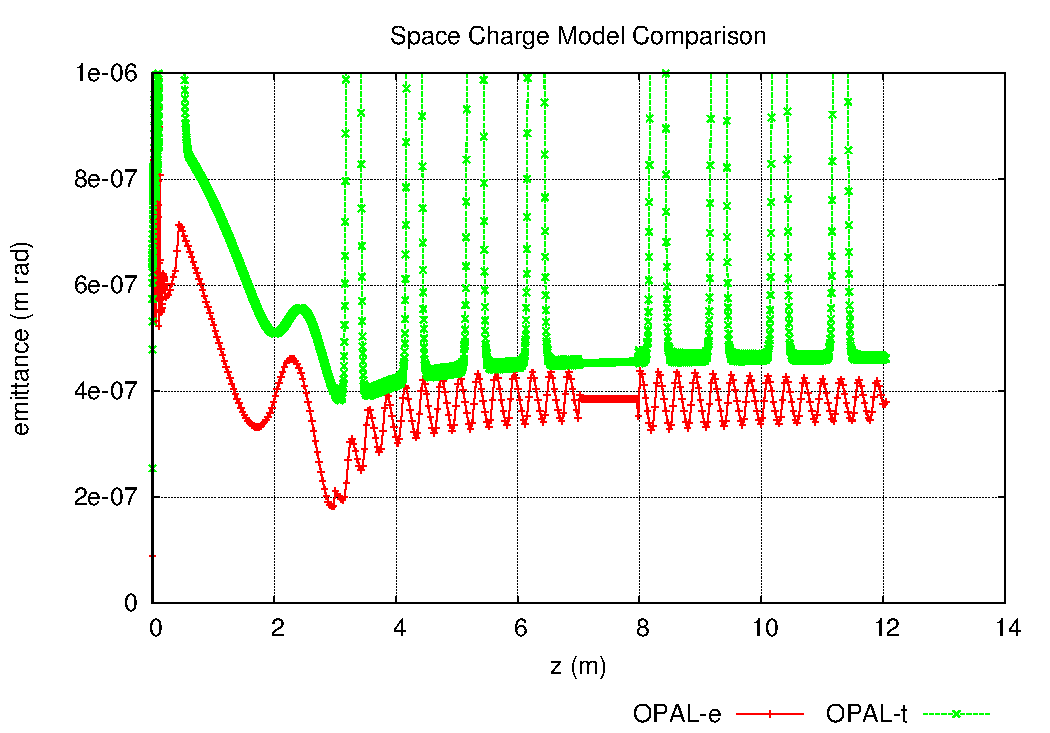
\includegraphics[width=0.45\textwidth]{figures/EMcompare}
      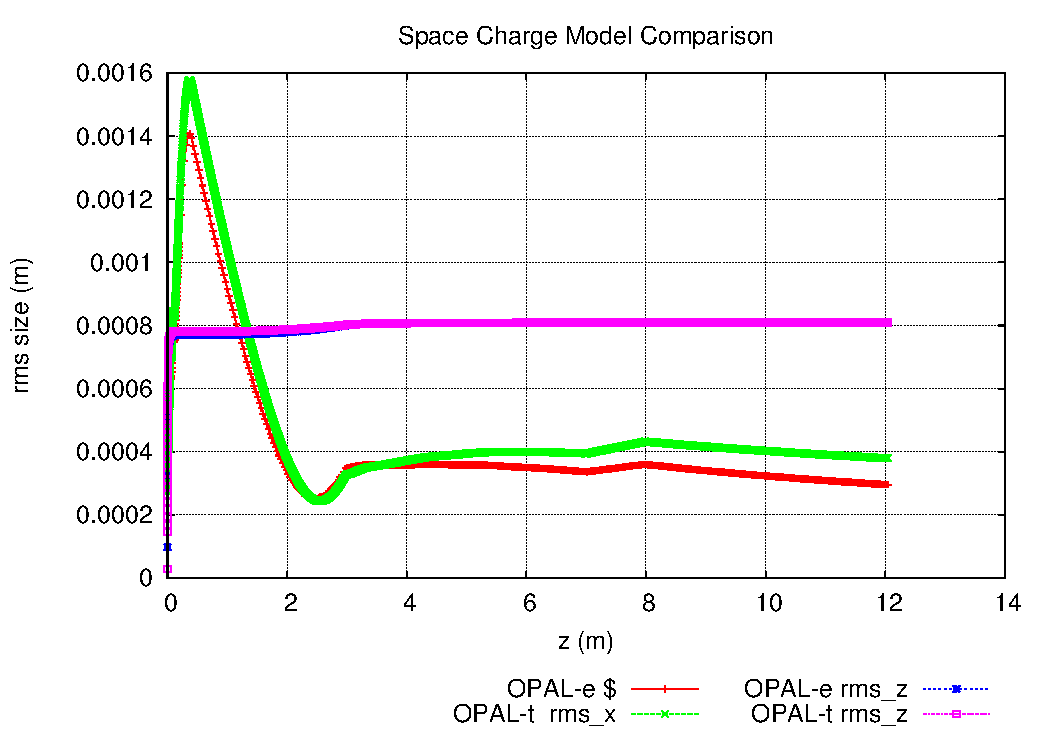
\includegraphics[width=0.45\textwidth]{figures/RMScompare}
    \end{center}
    \caption{%
    \label{fig:psiInjectorTest}
        Comparison of the \opalenv envelope tracker and the full 3D \opalt tracker
     in the first 12 meters of the \SI{250}{\mega\electronvolt} test injector at PSI. Shown here are
     both $\sigma_x$ and $\sigma_z$ (a), and the emittance (b).
     }%
\end{figure}
%
As both plots show, the agreement between both trackers is quite good. To
generate this data, the envelope tacker was run with 100 beam slices.